\documentclass[a4paper,12pt]{article}

\usepackage[utf8]{inputenc}
\usepackage[T1]{fontenc}
\usepackage[polish]{babel}
\usepackage{amsmath}
\usepackage{listings}
\usepackage{xcolor}
\usepackage{geometry}
\usepackage{float}
\usepackage{graphicx}
\usepackage{hyperref}

\geometry{margin=2.5cm}

\title{Implementacja perceptronu w podejściu obiektowym}
\author{Piotr Przymus 127902}
\date{}

\begin{document}

\maketitle

\section{Cel ćwiczenia}

Celem ćwiczenia było zaimplementowanie perceptronu w języku Python z wykorzystaniem podejścia obiektowego oraz sprawdzenie jego działania na przykładzie bramek logicznych AND oraz OR przy użyciu różnych funkcji aktywacji. Dodatkowo przeanalizowano możliwość realizacji bramki XOR.

\section{Podstawy teoretyczne}

Perceptron jest jednym z najprostszych modeli sztucznej sieci neuronowej. Jego działanie opiera się na obliczeniu sumy ważonej sygnałów wejściowych:

\[
z = w_1 x_1 + w_2 x_2 + b
\]

gdzie:
\begin{itemize}
\item $x_1$, $x_2$ -- dane wejściowe,
\item $w_1$, $w_2$ -- wagi,
\item $b$ -- bias.
\end{itemize}

Funkcja aktywacji decyduje o końcowym wyniku neuronu. Do funkcji aktywacji należą między innymi:
\begin{itemize}
\item funkcja progową (step),
\item sigmoid,
\item relu.
\end{itemize}

\section{Implementacja}

Zaimplementowano klasę \texttt{Perceptron}, która umożliwia:
\begin{itemize}
\item uczenie modelu (fit),
\item predykcję (predict),
\item ocenę skuteczności (evaluate).
\end{itemize}

Funkcja aktywacji została przekazana jako parametr konstruktora klasy.

\section{Eksperymenty}

W ramach eksperymentów przeanalizowano działanie perceptronu dla trzech bramek logicznych:
AND, OR oraz XOR. Dla każdej bramki porównano wyniki uzyskane przy użyciu trzech funkcji aktywacji:
step, sigmoid oraz relu.

% ==========================================================
\subsection{Bramka AND}

\begin{table}[H]
\centering
\begin{tabular}{c|c|c|c|c}
Wejście & Oczekiwany & Predykcja - step & Predykcja - sigmoid & Predykcja - relu\\
\hline
(0,0) & 0 & 0 & 0 & 0\\
(0,1) & 0 & 0 & 0 & 0\\
(1,0) & 0 & 0 & 0 & 0\\
(1,1) & 1 & 1 & 0 & 1\\
\end{tabular}
\end{table}

\textbf{Accuracy:}
\begin{itemize}
\item step: 1.0
\item sigmoid: 0.75
\item relu: 1.0
\end{itemize}

Model przy użyciu funkcji aktywacji step oraz relu poprawnie rozwiązuje problem bramki AND. Spadek jakości dla funkcji sigmoid wynika z ograniczeń progu decyzyjnego po stronie klasyfikacji binarnej.

% ==========================================================
\subsection{Bramka OR}

\begin{table}[H]
\centering
\begin{tabular}{c|c|c|c|c}
Wejście & Oczekiwany & Predykcja - step & Predykcja - sigmoid & Predykcja - relu\\
\hline
(0,0) & 0 & 0 & 1 & 0\\
(0,1) & 1 & 1 & 1 & 1\\
(1,0) & 1 & 1 & 1 & 1\\
(1,1) & 1 & 1 & 1 & 1\\
\end{tabular}
\end{table}

\textbf{Accuracy:}
\begin{itemize}
\item step: 1.0
\item sigmoid: 0.75
\item relu: 1.0
\end{itemize}

Podobnie jak dla bramki AND, perceptron z funkcjami aktywacji step i relu poprawnie rozwiązuje problem bramki OR, a funkcja sigmoid radzi sobie gorzej.

% ==========================================================
\subsection{Bramka XOR}

\begin{table}[H]
\centering
\begin{tabular}{c|c|c|c|c}
Wejście & Oczekiwany & Predykcja - step & Predykcja - sigmoid & Predykcja - relu\\
\hline
(0,0) & 0 & 1 & 0 & 0\\
(0,1) & 1 & 1 & 0 & 0\\
(1,0) & 1 & 0 & 0 & 0\\
(1,1) & 0 & 0 & 0 & 0\\
\end{tabular}
\end{table}

\textbf{Accuracy:}
\begin{itemize}
\item step: 0.5
\item sigmoid: 0.5
\item relu: 0.5
\end{itemize}

Niezależnie od użytej funkcji aktywacji perceptron nie był w stanie poprawnie nauczyć się
pełnej zależności wejście-wyjście dla bramki XOR. Wynika to z faktu, że problem XOR nie jest liniowo separowalny, co jest fundamentalnym ograniczeniem perceptronu jednowarstwowego.

% ==========================================================
\section{Analiza problemu XOR}

Model działa bardzo dobrze dla problemów liniowo separowalnych, takich jak bramki AND oraz OR. Oznacza to, że da się znaleźć jedną prostą (w praktyce: linię na wykresie), która oddziela przypadki należące do klasy 0 i 1.

W przypadku bramki XOR sytuacja jest inna. Dane wejściowe XOR mają taką strukturę, że nie da się ich rozdzielić jedną prostą linią. Jeśli narysujemy punkty (0,0), (0,1), (1,0), (1,1), to klasy 0 i 1 są „przeplatane” po przekątnej. Oznacza to, że każda pojedyncza linia podziału zawsze pomyli przynajmniej jeden punkt.

Perceptron jednowarstwowy działa dokładnie w taki sposób, że podejmuje decyzję na podstawie jednej takiej linii (hiperpłaszczyzny) opisanej równaniem:
\[
w_1x_1 + w_2x_2 + b = 0
\]

Dlatego niezależnie od tego, jak dobierzemy wagi, bias albo funkcję aktywacji, model nadal próbuje oddzielić dane jedną prostą granicą decyzyjną. To powoduje, że nie jest w stanie poprawnie nauczyć się XOR.

W praktyce oznacza to, że problem nie leży w implementacji ani w funkcji aktywacji, tylko w samej architekturze modelu - jest ona zbyt prosta. Jak można zaobserwować na rysunku \ref{fig:xor}, klasy XOR nie mogą zostać rozdzielone jedną linią prostą. Aby uzyskać poprawną separację, konieczne jest zastosowanie co najmniej dwóch linii decyzyjnych, co wykracza poza możliwości pojedynczego perceptronu. Z tego powodu do rozwiązania XOR potrzebna jest sieć neuronowa z co najmniej jedną warstwą ukrytą, która potrafi tworzyć bardziej złożone, nieliniowe granice decyzyjne.

\begin{figure}[H]
\centering
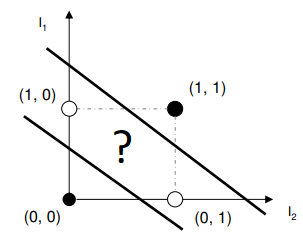
\includegraphics[width=0.62\textwidth]{xor.png}
\caption{Wizualizacja problemu XOR. Punkty (0,0) i (1,1) należą do klasy 0, a punkty (0,1) i (1,0) należą do klasy 1. Nie można oddzielić tych klas jedną prostą linią.}
\label{fig:xor}
\end{figure}

% ==========================================================
\section{Wnioski}

\begin{enumerate}
\item Perceptron został poprawnie zaimplementowany i działa zgodnie z założeniami teoretycznymi. Potrafi uczyć się na podstawowych danych wejściowych i dostosowywać wagi oraz bias.

\item Model bardzo dobrze radzi sobie z prostymi problemami, które można rozdzielić jedną linią, takimi jak bramki AND oraz OR. W takich przypadkach osiąga wysoką skuteczność niezależnie od funkcji aktywacji.

\item Funkcje aktywacji step, sigmoid oraz relu wpływają na sposób działania modelu, jednak nie zmieniają jego podstawowych ograniczeń. W niektórych przypadkach sigmoid może pogarszać wyniki w zadaniach binarnych.

\item Problem XOR nie został poprawnie rozwiązany przez perceptron, ponieważ dane nie są liniowo separowalne. Oznacza to, że nie da się ich poprawnie rozdzielić jedną prostą granicą decyzyjną.

\item Najważniejszym ograniczeniem perceptronu nie jest funkcja aktywacji, ale jego liniowa struktura, która pozwala na tworzenie tylko prostych granic decyzyjnych.

\item Aby rozwiązać bardziej złożone problemy, takie jak XOR, konieczne jest zastosowanie bardziej zaawansowanych modeli, np. sieci neuronowych z warstwami ukrytymi.
\end{enumerate}

\end{document}